\documentclass[12pt,a4paper]{article}
\usepackage[a4paper, left=2.5cm,right=2.5cm,top=3cm,bottom=3cm]{geometry}
\usepackage[utf8]{inputenc}
\usepackage[spanish]{babel}
\addto\captionsspanish{
	\renewcommand\chaptername{}
	\renewcommand\appendixname{Anexo}
	\renewcommand\appendixpagename{Anexos}
	\def\tablename{Tabla}
	\def\listtablename{\'Indice de tablas}
}
\usepackage{ucs}
\usepackage{subfig}
\usepackage{float}
\usepackage{amsmath}
\usepackage{amsfonts}
\usepackage{amssymb}
\usepackage{graphicx}
\usepackage{listings}
\usepackage{color}
\usepackage[T1]{fontenc}
\usepackage[scaled]{beramono}
\usepackage{upquote}
\usepackage{xcolor}
\usepackage{listings}
\usepackage{caption}
\usepackage{chngcntr}
\usepackage{endnotes}
\usepackage{float}
\usepackage{hyperref}
\usepackage{wrapfig}
\usepackage{fancyhdr}
\usepackage{emptypage}
\usepackage{times}
\usepackage{array}
\usepackage{setspace}
\usepackage{multirow}
%\usepackage{subfigure}
\usepackage{verbatim}
%\usepackage{tabulary}
%\usepackage{graphicx,subfigure}
\usepackage[bottom]{footmisc} 
\usepackage{appendix}
\usepackage{mathtools}
\usepackage{textcomp}


%listing, code style
% Define a custom color
\definecolor{backcolour}{rgb}{0.95,0.95,0.92}
\definecolor{codegreen}{rgb}{0,0.6,0}

% Define listing style
\lstset{
	language=python,
	tabsize=4,
	rulecolor=,
	basicstyle=\scriptsize,
	upquote=true,
	aboveskip={1.2\baselineskip},
	columns=fixed,
	numbers=left,
	showstringspaces=false,
	extendedchars=true,
	breaklines=true,
	prebreak = \raisebox{0ex}[0ex][0ex]{\ensuremath{\hookleftarrow}},
	showtabs=false,
	showspaces=false,
	showstringspaces=false,
	identifierstyle=\ttfamily,
	keywordstyle=\color[rgb]{0,0,1},
	commentstyle=\color[rgb]{0.133,0.545,0.133},
	stringstyle=\color[rgb]{0.627,0.126,0.941},
} 


\renewcommand{\notesname}{Fuentes}
\renewcommand{\baselinestretch}{1.2}
\hypersetup{
	colorlinks,%
	citecolor=black,%
	filecolor=black,%
	linkcolor=black,%
	urlcolor=black
}

\begin{document}
	
\begin{titlepage}
	\centering
	%\null\vfill
	
\includegraphics[width=\textwidth]{FIGURES/Portada/Logo_portada.png} 
	\vspace{1.5cm}
	
	Universidad Politécnica de Madrid
	\\Escuela Técnica Superior de Ingeniería Aeronáutica y del Espacio
	\vspace{2cm}
	
	{\large MÁSTER UNIVERSITARIO EN SISTEMAS ESPACIALES}
	\vspace{2cm}
	
	{\LARGE MILESTONE 3}
	\vspace{1cm}
	
	{\large Ampliación de Matemáticas I}
	\vspace{4cm}
	
	\begin{center}
		\large{\textbf{\today}} \\
	\end{center}
	
	Autor: \\ Alberto García Rincón
	\vfill
\end{titlepage}

%****INDICES****
\newpage
\pagestyle{empty}
\tableofcontents	

%******DOC******	
\newpage
\pagenumbering{arabic}
\setcounter{page}{1}
\pagestyle{fancy} 

\section{Introducción}
Como continuación del ejercicio resuelto la semana pasada, en este trabajo se ha implementado el método de extrapolación de Richardson para evaluar el el error de los distintos métodos de cálculo numérico que ya que habían programado en el ejercicio anterior. Posteriormente se ha programado una función que evalúa el ratio de convergencia de dichos métodos de cálculo numérico. 


\section{Código de Python}
La estructura de división de cada función en archivos distintos se mantiene para este trabajo, puesto que es la forma correcta de programar.

Se ha creado dos funciones para calcular el error numérico mediante la extrapolación de Richardson y otra para calcular el ratio de convergencia de los respectivos métodos de cálculo que ya se habían implementado en el trabajo anterior. Todas las funciones relativas a la creación de las gráficas están en otro archivo distinto denominado \textit{plots.py}.

Solo se mostrarán y se realizará un breve análisis de las funciones nuevas creadas para este trabajo, así como las modificaciones o reestructura de código de algunos archivos. 

\subsection{\textit{milestone\_3.py}}
Respecto al programa principal se ha reescrito el proceso de llamar al resto de funciones para calcular los distintos vectores de elementos que se piden para este trabajo. Ahora se ejecuta un bucle que recorre los distintos métodos implementados y en cada paso se calculan las distintas instancias (vector de estado, error y ratio de convergencia) que se piden.
\begin{figure}[H] 
	\centering
	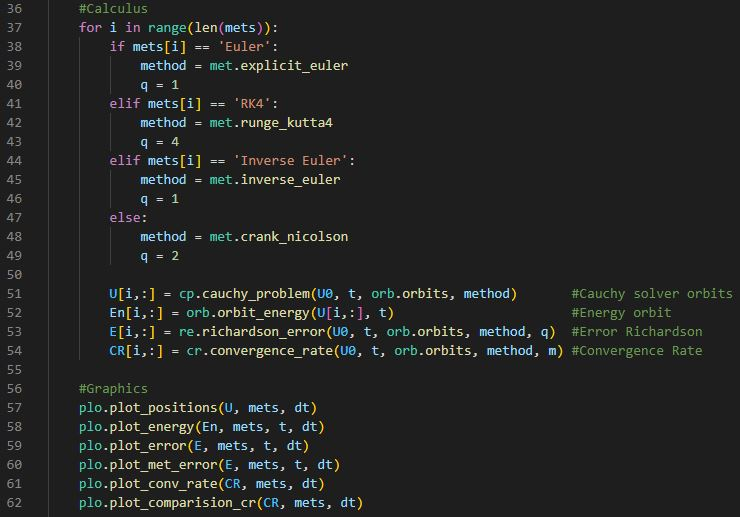
\includegraphics[width=0.9\textwidth]{FIGURES/Codigo/main_milestone3.jpg}
	\caption{\textit{milestone3.py}.}
\end{figure}

\subsection{\textit{richardson\_error.py}}
Esta función tiene como argumentos el vector de estado inicial, el vector de tiempo donde se va a implementar la simulación, la función que define el comportamiento del objeto de estudio, el método que se va a usar para el cálculo de su comportamiento y el orden del método numérico.

La función nos devuelve una matriz que contiene todos los errores estimados para cada intervalo de tiempo para cada una de las variables de estado. El error asociado a cada variable esta definido en una fila.
\begin{figure}[H] 
	\centering
	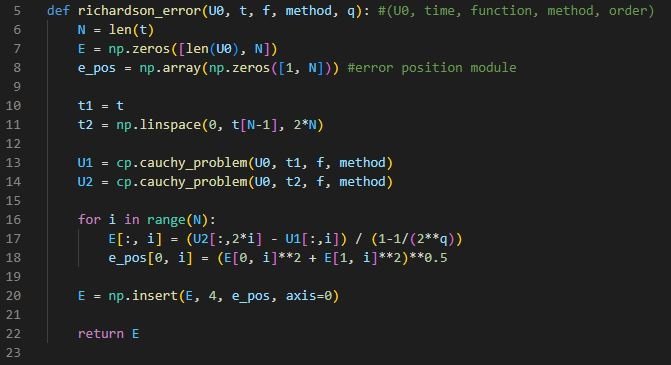
\includegraphics[width=0.8\textwidth]{FIGURES/Codigo/richardson_error.jpg}
	\caption{\textit{richardson\_error.py}.}
\end{figure}
Se ha añadido una fila más a la matriz que devuelve la función: el módulo del error de la posición, es decir, el módulo entre las dos variables de estado que definen la posición para cada intervalo de tiempo, calculado en la misma función como: \textit{e\_pos}.

\subsection{\textit{convergence\_rate.py}}
Esta función necesita como argumentos el vector de estado inicial, el vector que define el tiempo de la simulación, la función que define el comportamiento del objeto de estudio, el método de cálculo numérico y el número de puntos que se van a utilizar para calcular la convergencia.
\begin{figure}[H] 
	\centering
	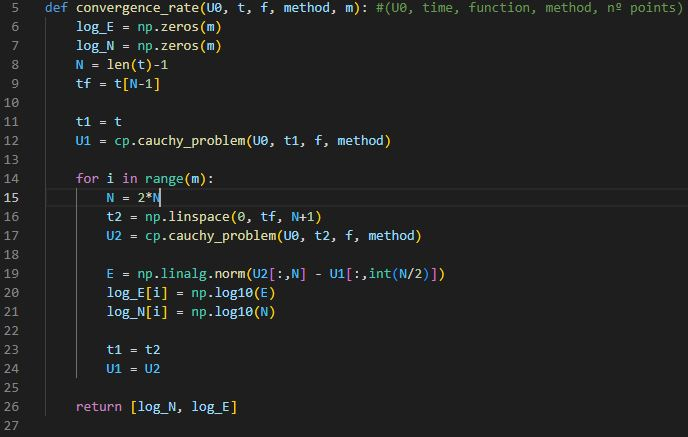
\includegraphics[width=0.8\textwidth]{FIGURES/Codigo/convergence_rate.jpg}
	\caption{\textit{convergence\_rate.py}.}
\end{figure}



\section{Resultados de los métodos}
Se ha fijado un tiempo total de simulación de 30 segundos se han realizado varias simulaciones con distintos $\Delta t$ para comprobar que el código funciona correctamente. Aquí solo se muestran algunas de esas simulaciones.

\subsection{Error por extrapolación de Richardson}
Este método permite la estimación del error de cálculo que se obtiene utilizando un método de resolución. Para este trabajo se ha calculado el error utilizando los cuatro métodos de resolución siguientes: Euler explícito, Runge-Kutta de orden 4, Euler inverso y Crank-Nicholson. El método consiste en evaluar la solución en dos mallas temporales con diferente intervalo de tiempo, una de ellas con el mismo intervalo que la resolución con el método de cálculo y la otra con un intervalo la mitad del anterior. La ecuación que define la estimación del error por la extrapolación de Richardson es:
\begin{equation} 
	E = \frac{U^{2N} - U^{N}}{1 - \frac{1}{2^{q}}}
\end{equation} 
siendo q el orden de integración del método de cálculo utilizado.

\subsubsection{Simulaciones con: $\Delta t = 0.1 s$}
Como se puede observar en la figura de abajo con un intervalo de integración alto, se obtienen errores considerables. La tendencia creciente del error en la posición en todos los métodos es notable puesto que según se va avanzando en el tiempo de simulación se va acumulando el error de la integración anterior.
\begin{figure}[H] 
	\centering
	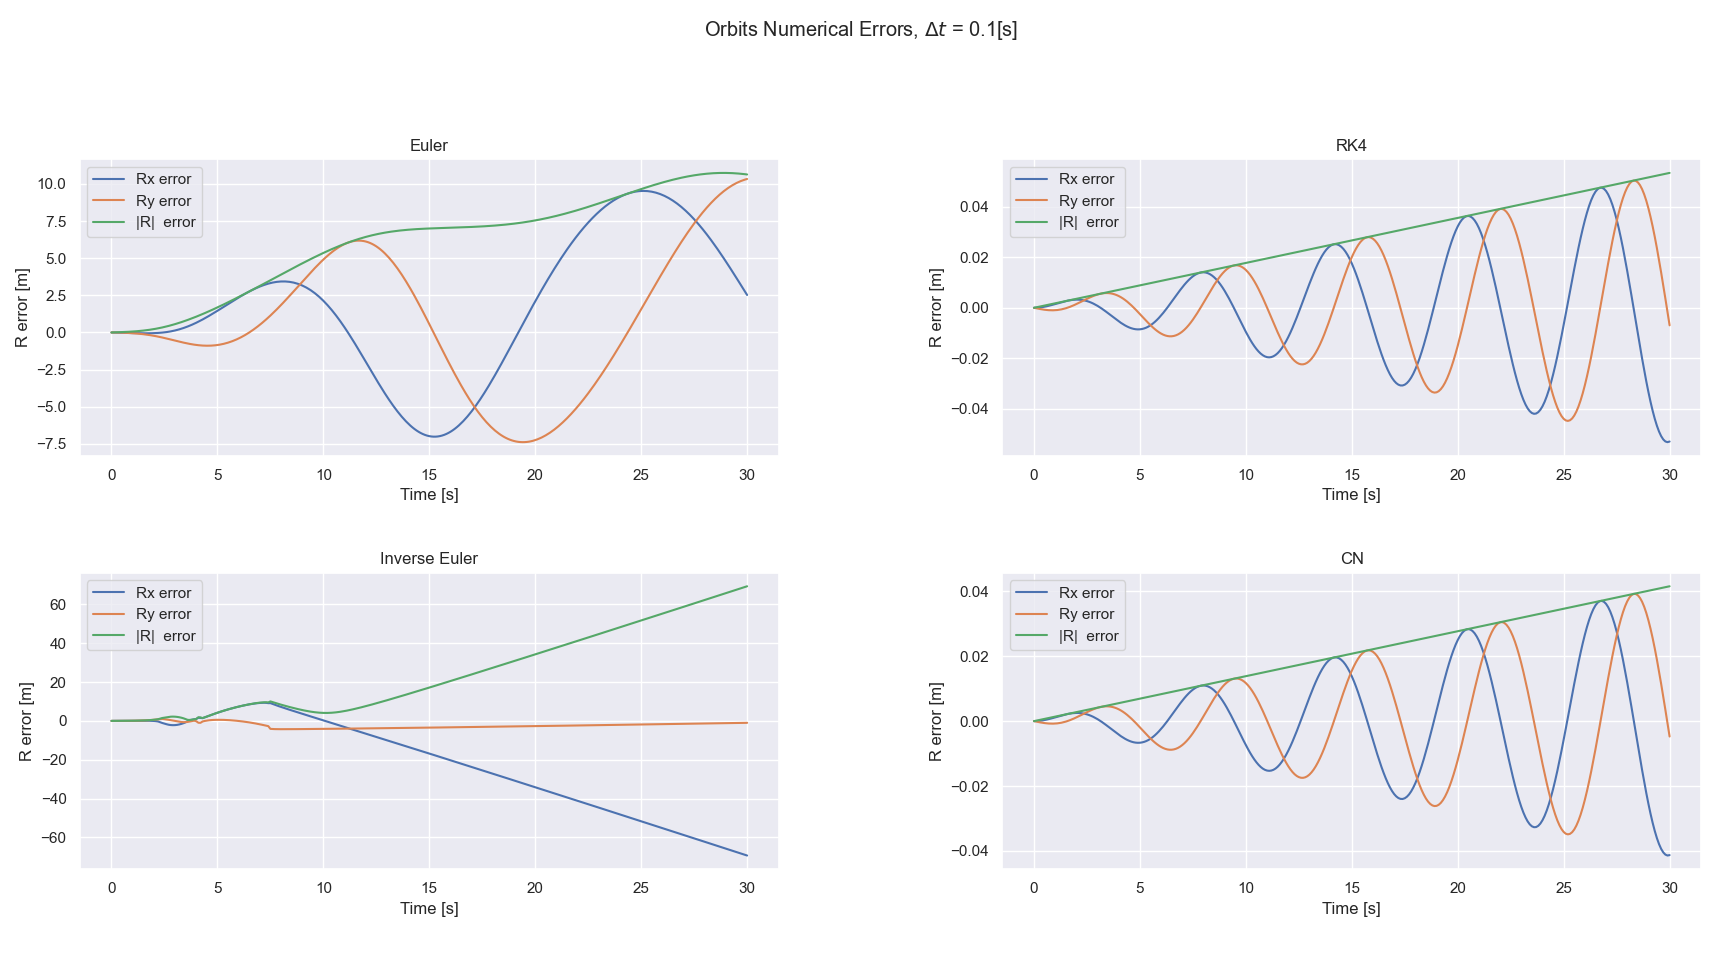
\includegraphics[width=0.95\textwidth]{FIGURES/dt0.1_error.png}
	\caption{Errores de posición de los distintos métodos.}
\end{figure}

En la siguiente figura se  observa una comparación entre los módulos de error de posición estimados para los distintos métodos de cálculo.

Cabe mencionar que con los métodos de orden superior (Runge-Kutta y Crank-Nicholson) se obtienen errores de posición menores que con el método de Euler. En el caso del método de Euler inverso, el error se dispara a los 10 segundos de la simulación debido a que en ese tiempo ha convergido su solución a cero y no estaría funcionando correctamente, para solucionarlo se debe disminuir el intervalo de tiempo con el que se realiza la simulación.
\begin{figure}[H] 
	\centering
	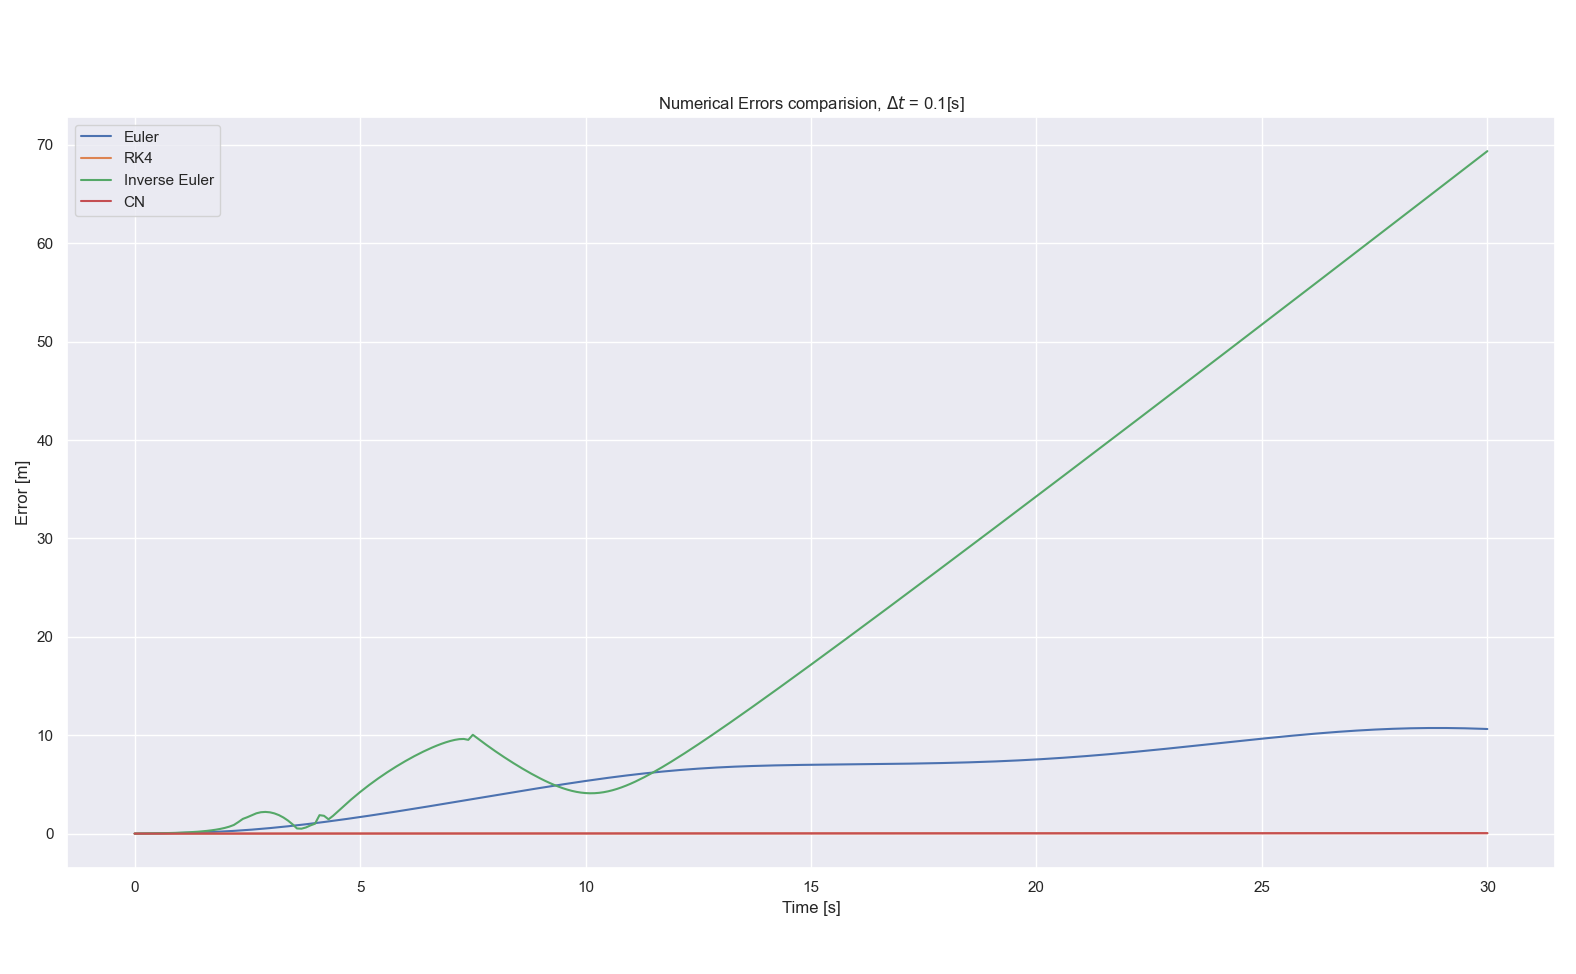
\includegraphics[width=0.95\textwidth]{FIGURES/dt0.1_error_comparison.png}
	\caption{Comparación del módulo de error de la posición entre los distintos métodos.}
\end{figure}


\subsubsection{Simulaciones con: $\Delta t = 0.001 s$}
En esta simulación se obtienen mejoras relativas de cada método respecto a la simulación anterior.
En la figura siguiente se han representado los errores estimados de posición a lo largo del tiempo de simulación.
\begin{figure}[H] 
	\centering
	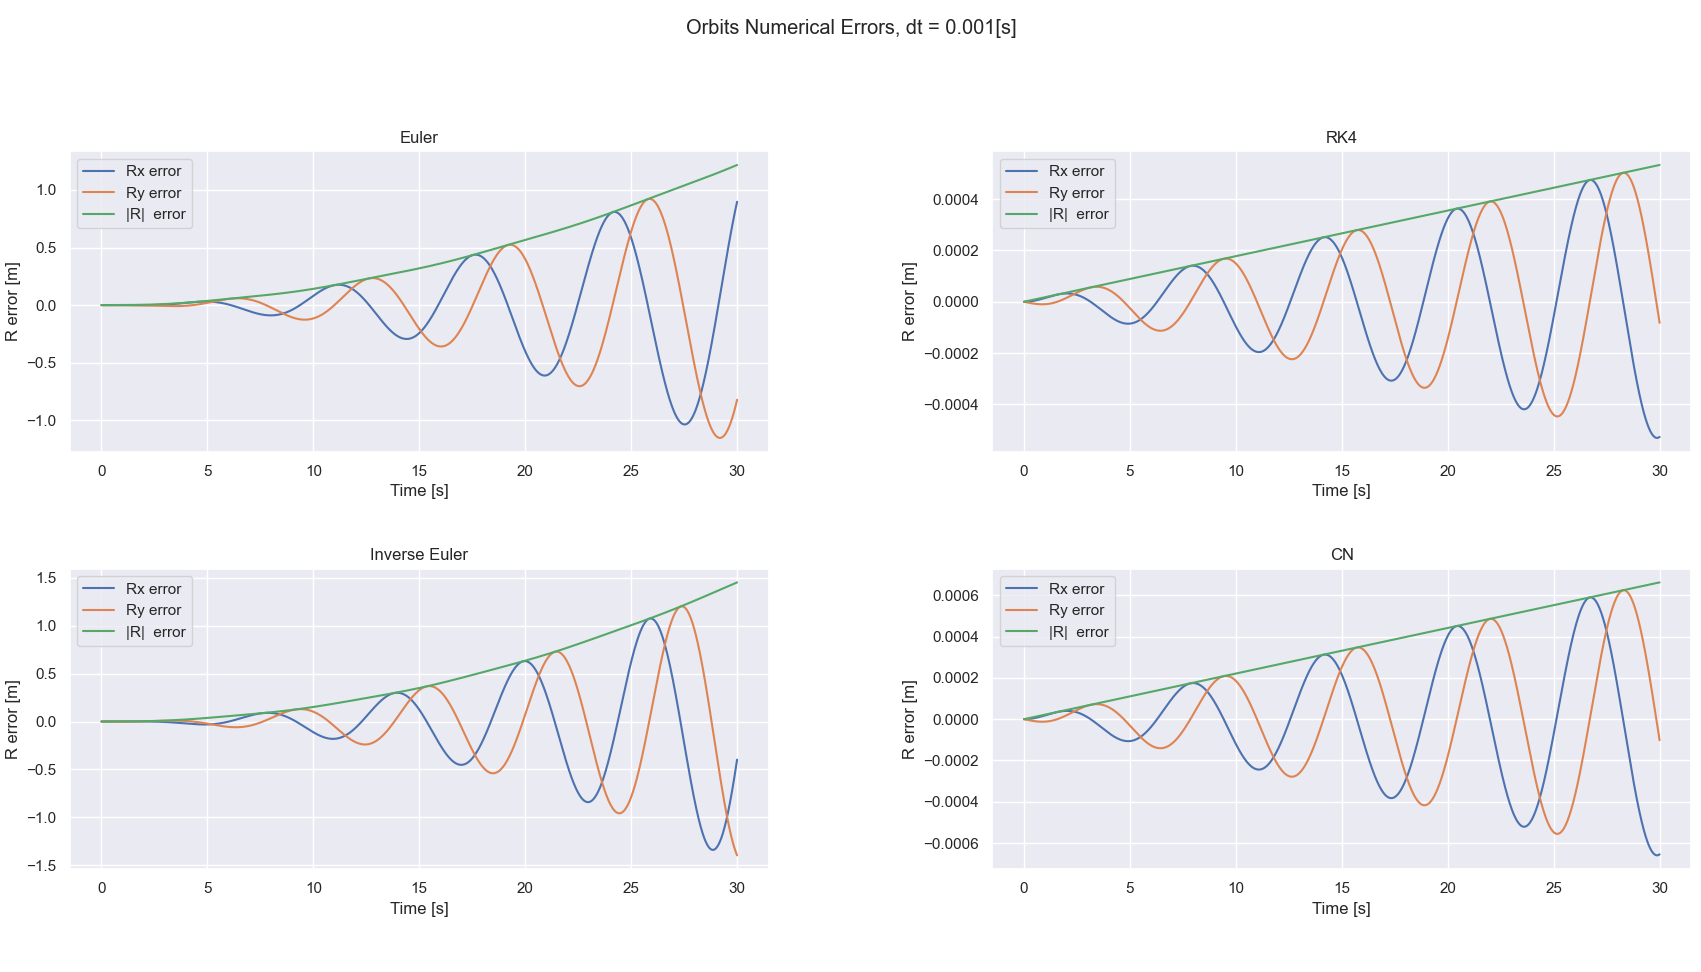
\includegraphics[width=0.95\textwidth]{FIGURES/dt0.001_error.png}
	\caption{Errores de posición de los distintos métodos.}
\end{figure}

En esta otra figura se comparan los módulos de error de posición estimados. En este caso, al igual que en el anterior, los métodos de Crank-Nicholson y Runge-Kutta generan menos error que los métodos de Euler y de Euler inverso. 

Para esta simulación, con el intervalo de tiempo utilizado ($\Delta t = 0.001 s$), ha quedado solucionado el problema de la anterior simulación con el método de Euler inverso. 
\begin{figure}[H] 
	\centering
	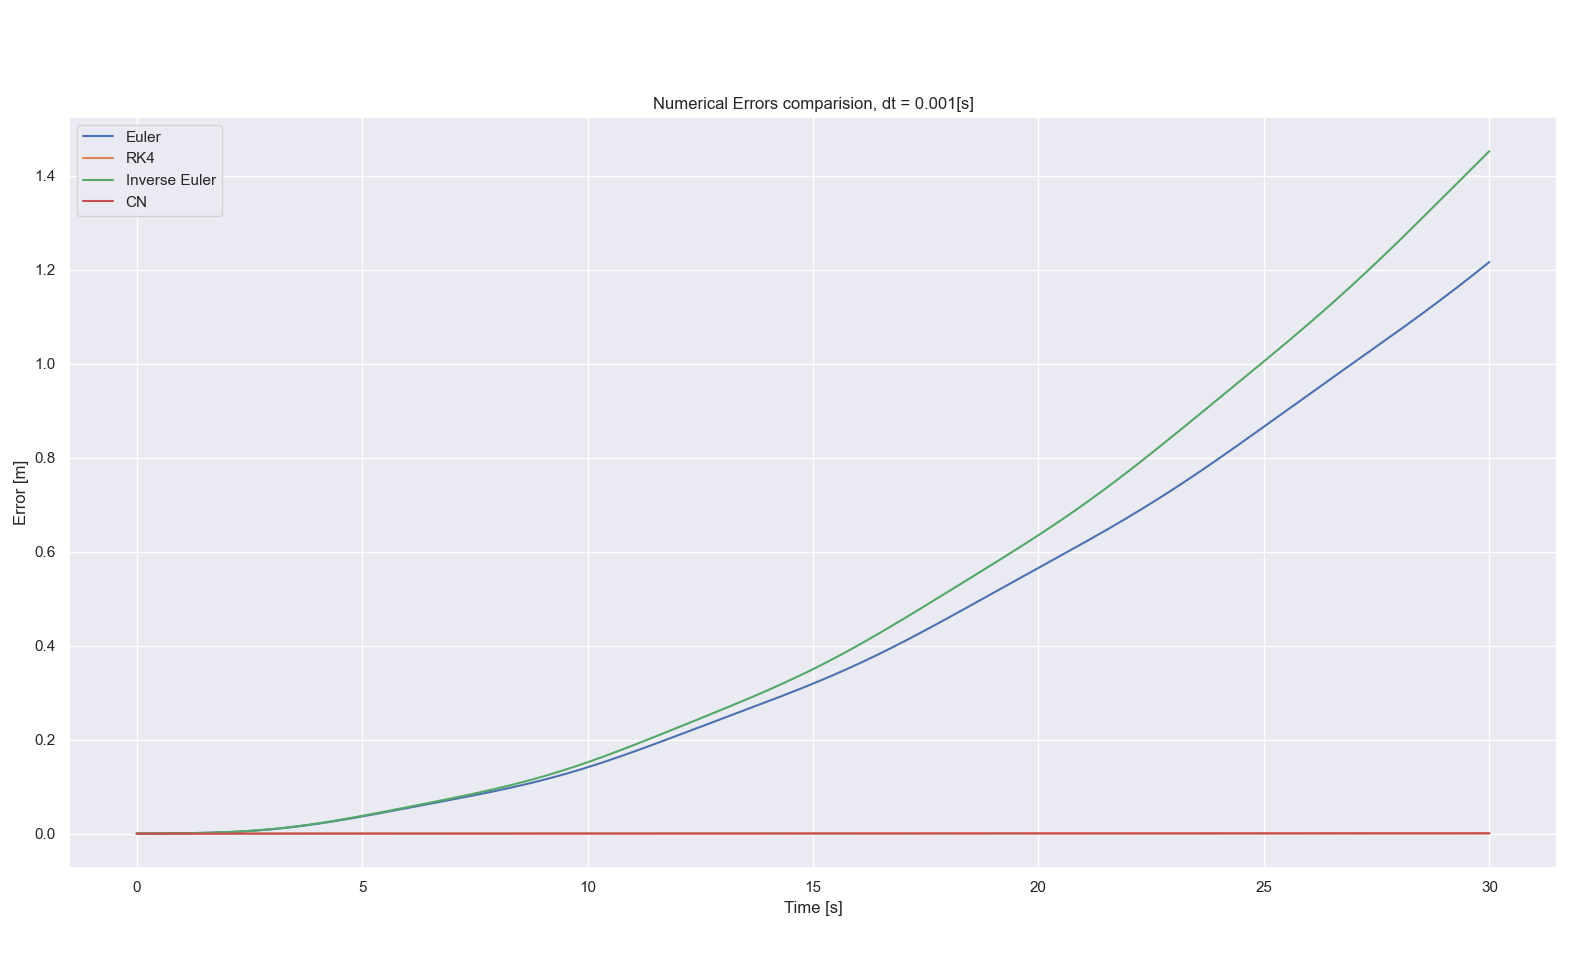
\includegraphics[width=0.95\textwidth]{FIGURES/dt0.001_error_comparison.png}
	\caption{Comparación del módulo de error de la posición entre los distintos métodos.}
\end{figure}

\subsection{Ratio de convergencia}
Permite obtener el orden de integración de un método de cálculo numérico. Se representa gráficamente el logaritmo del error estimado con el método de la extrapolación de Richardson $log(|U^{2N} - U^{N}|)$ frente al logaritmo del número de puntos de integración $log(N)$. La pendiente de dicha gráfica es el orden de integración práctico.

\subsubsection{Simulaciones con: $\Delta t = 0.1 s$}
Se observa que para simulaciones con incrementos de tiempo elevados el orden de integración se aleja del teórico, sobre todo en los métodos de Euler y de Euler inverso. 
\begin{figure}[H] 
	\centering
	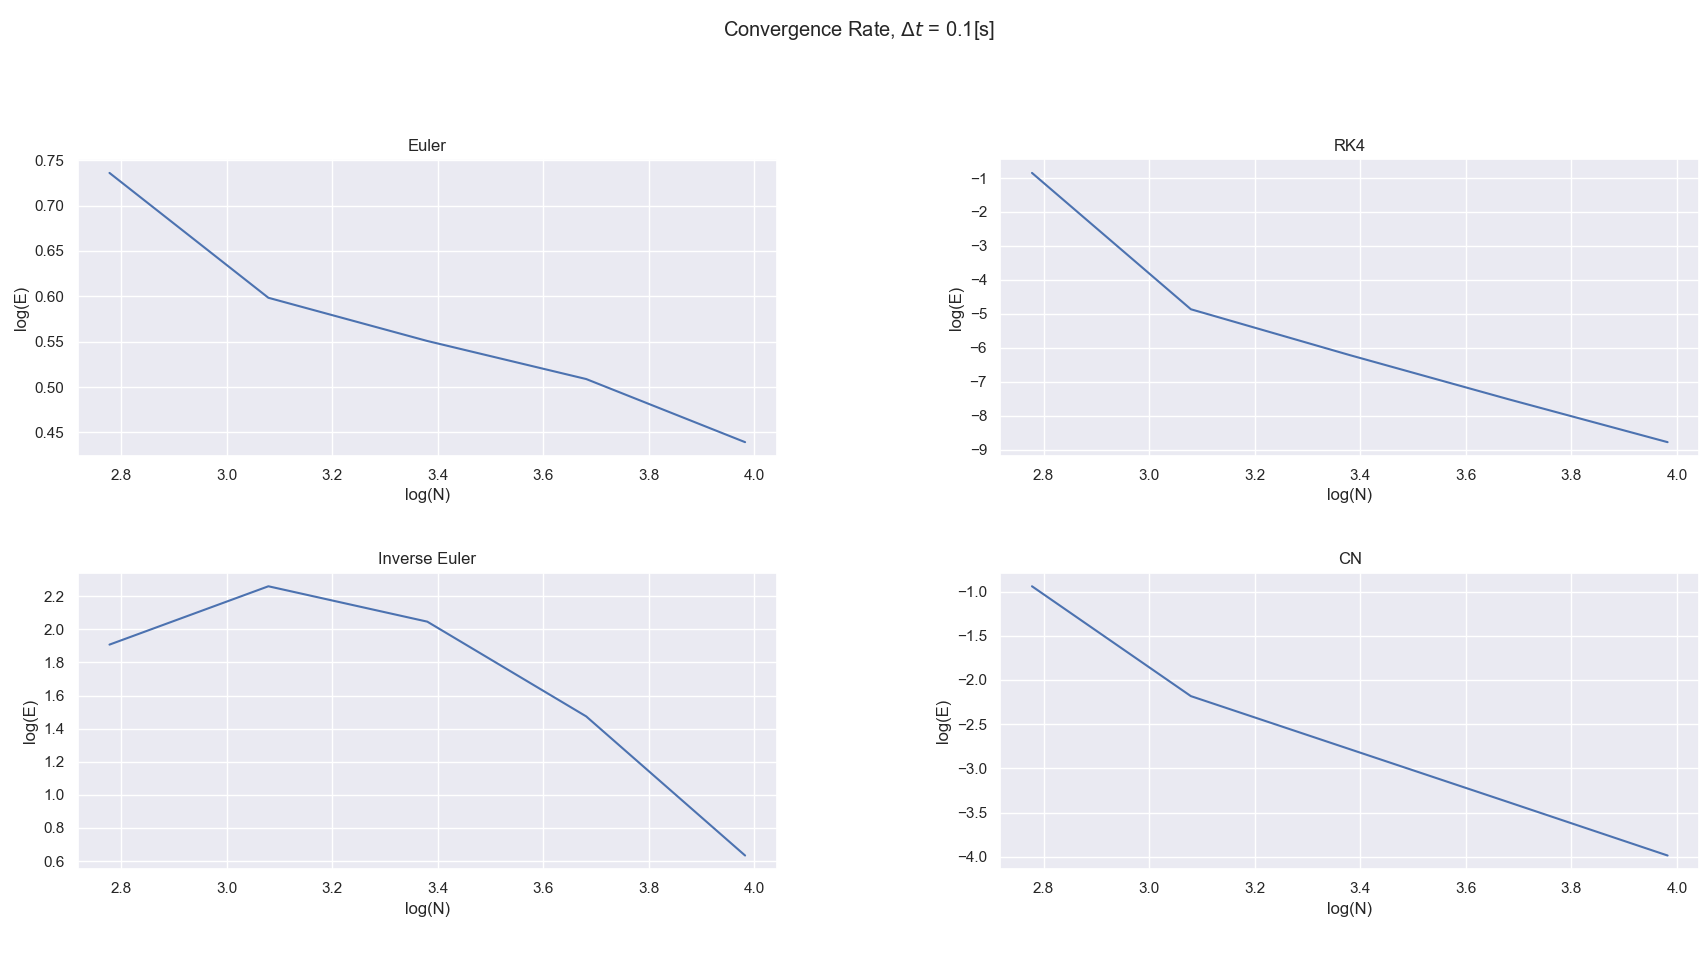
\includegraphics[width=0.95\textwidth]{FIGURES/dt0.1_convergence.png}
	\caption{Ratio de convergencia de los distintos métodos.}
\end{figure}


\subsubsection{Simulaciones con: $\Delta t = 0.001 s$}
Conforme se disminuye el $\Delta t$, los puntos obtenidos forman una recta más definida cuya pendiente corresponde con el orden del esquema numérico.

Para el método de Euler se puede calcular la pendiente de la recta de la figura de abajo, siendo aproximadamente $-1$, correspondiéndose en valor absoluto con el orden del método.

Para el resto de métodos se pueden obtener las pendientes de las rectas y se obtendrían conclusiones similares, pero con a su orden de integración.
\begin{figure}[H] 
	\centering
	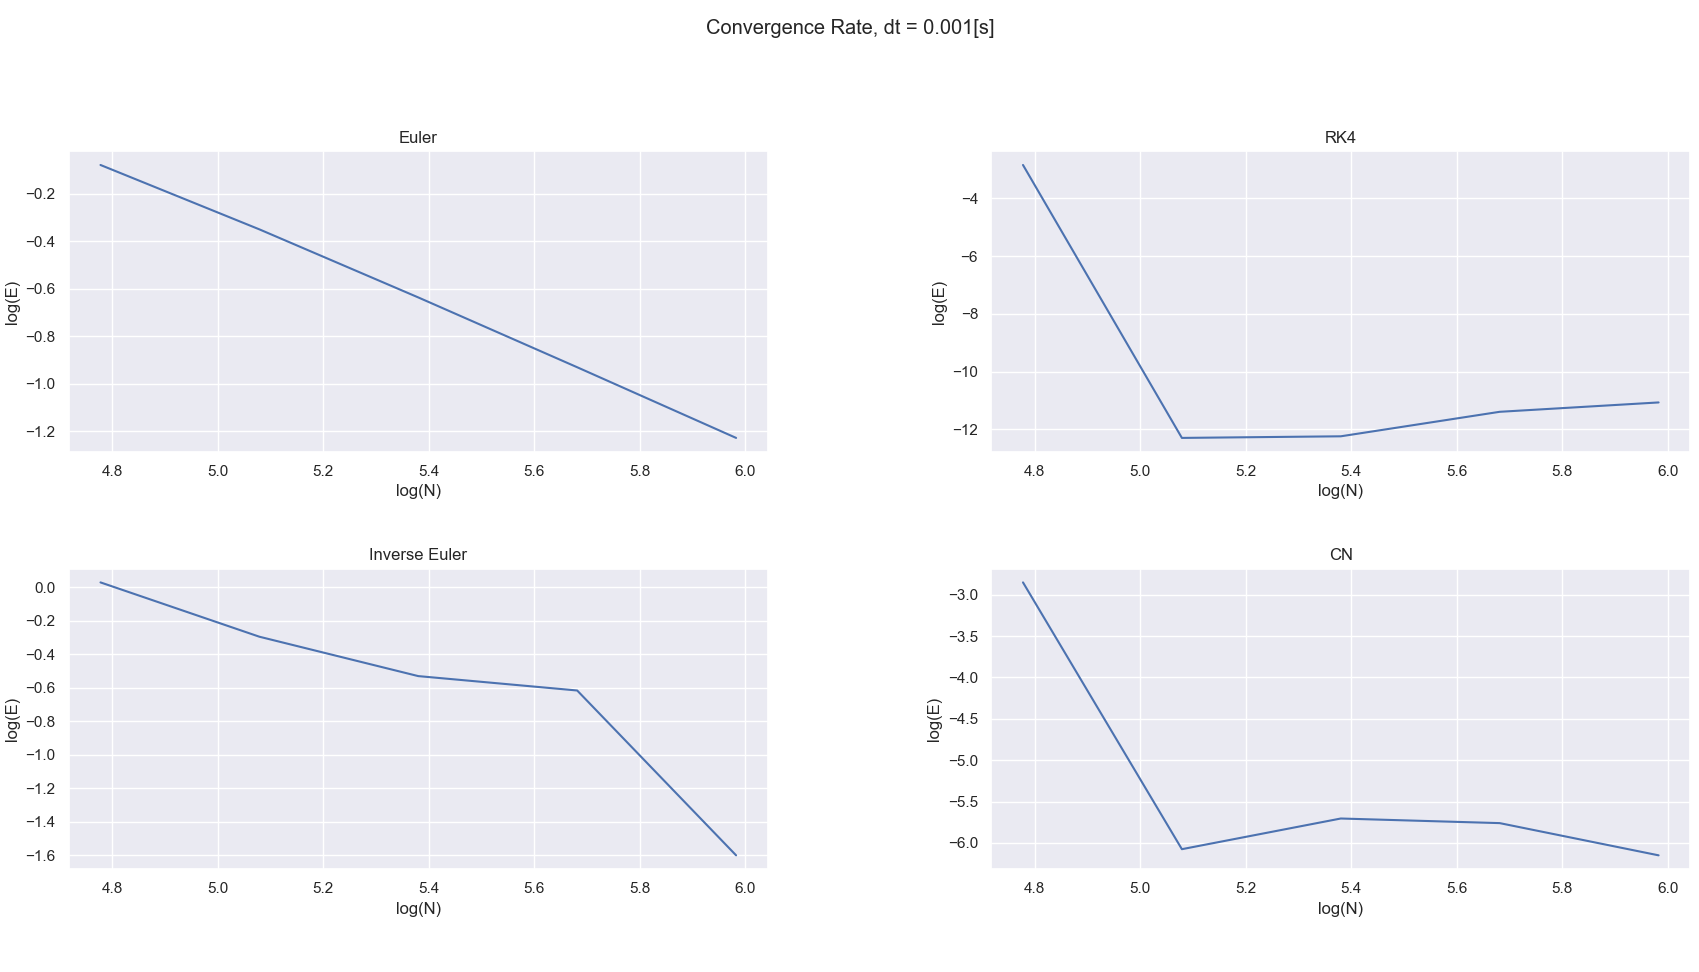
\includegraphics[width=0.95\textwidth]{FIGURES/dt0.001_convergence.png}
	\caption{Ratio de convergencia de los distintos métodos.}
\end{figure}

\end{document}
